\documentclass[tikz, border=2pt]{standalone}
\usepackage{amsmath}

\begin{document}
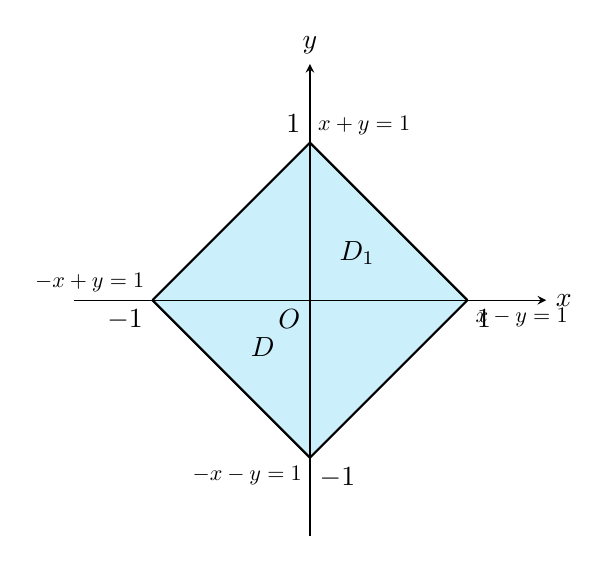
\begin{tikzpicture}[scale=2, >=stealth]
    % 填充积分区域 D (正方形：|x| + |y| <= 1)
    \fill[cyan!20] (1,0) -- (0,1) -- (-1,0) -- (0,-1) -- cycle;

    % 画坐标轴
    \draw[->] (-1.5, 0) -- (1.5, 0) node[right] {$x$};
    \draw[->] (0, -1.5) -- (0, 1.5) node[above] {$y$};

    % 画边界线条
    \draw[thick] (1,0) -- (0,1) node[above right, scale=0.8] {$x+y=1$};
    \draw[thick] (0,1) -- (-1,0) node[above left, scale=0.8] {$-x+y=1$};
    \draw[thick] (-1,0) -- (0,-1) node[below left, scale=0.8] {$-x-y=1$};
    \draw[thick] (0,-1) -- (1,0) node[below right, scale=0.8] {$x-y=1$};

    % 标注关键坐标点
    \node[below right] at (1,0) {$1$};
    \node[above left] at (0,1) {$1$};
    \node[below left] at (-1,0) {$-1$};
    \node[below right] at (0,-1) {$-1$};
    \node[below left] at (0,0) {$O$};

    % 标注区域 D
    \node at (-0.3, -0.3) {$D$};
    \node at (0.3, 0.3) {$D_1$};
\end{tikzpicture}
\end{document}